% The Riesz diagram for the Fourier transform. Generated by a short script.
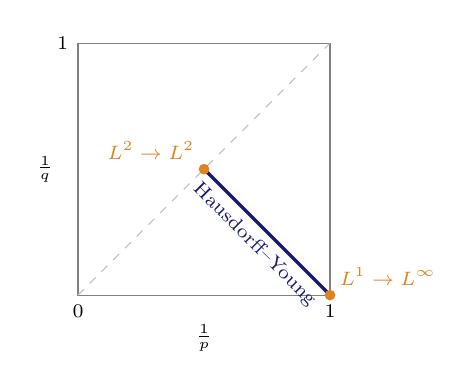
\begin{tikzpicture}[scale=3.2]
\draw[black!50] (0,0) rectangle (1,1);
\node[below,font=\scriptsize] at (0,0) {$0$};
\node[below,font=\scriptsize] at (1,0) {$1$};
\node[left,font=\scriptsize] at (0,1) {$1$};
\node[below,font=\scriptsize] at (0.5,-0.08) {$\frac1p$};
\node[left,font=\scriptsize] at (-0.06,0.5) {$\frac1q$};
\draw[black!25,dashed] (0,0) -- (1,1);
\draw[MidnightBlue,very thick] (1,0) -- (0.5,0.5);
\fill[BurntOrange!90!black] (1,0) circle (0.6pt) node[above right,font=\scriptsize] {$L^1\to L^\infty$};
\fill[BurntOrange!90!black] (0.5,0.5) circle (0.6pt) node[above left,font=\scriptsize] {$L^2\to L^2$};
\node[MidnightBlue,font=\scriptsize,rotate=-45] at (0.70,0.20) {Hausdorff--Young};
\end{tikzpicture}
